\documentclass[lettersize,journal]{IEEEtran}
\usepackage{amsmath,amsfonts}
\usepackage{algorithmic}
\usepackage{algorithm}
\usepackage{array}
\usepackage[caption=false,font=normalsize,labelfont=sf,textfont=sf]{subfig}
\usepackage{textcomp}
\usepackage{stfloats}
\usepackage{url}
\usepackage{verbatim}
\usepackage{graphicx}
\usepackage{cite}
\usepackage{booktabs}
\usepackage{hyperref}
\usepackage{multirow}
\hyphenation{op-tical net-works semi-conduc-tor IEEE-Xplore}
% updated with editorial comments 8/9/2021

\begin{document}

\title{Learning Annotation-Driven Latent Structure for Multi-Modal Fusion}

\author{
Meilun Zhou,~\IEEEmembership{Graduate Student Member, IEEE},
Aditya Dutt~\IEEEmembership{Member, IEEE},
Alina Zare,~\IEEEmembership{Senior Member, IEEE}%
\thanks{
Meilun Zhou, Aditya Dutt, and Alina Zare are with the Department of Electrical and Computer Engineering, University of Florida, Gainesville, FL, USA.
}%
\thanks{
Alina Zare is also with the Artificial Intelligence and Informatics Research Institute, University of Florida, Gainesville, FL, USA.
}%
}



%         % <-this % stops a space
% \thanks{This paper was produced by the IEEE Publication Technology Group. They are in Piscataway, NJ.}% <-this % stops a space
% \thanks{Manuscript received April 19, 2021; revised August 16, 2021.}}

% % The paper headers
% \markboth{Journal of \LaTeX\ Class Files,~Vol.~14, No.~8, August~2021}%
% {Shell \MakeLowercase{\textit{et al.}}: A Sample Article Using IEEEtran.cls for IEEE Journals}

% \IEEEpubid{0000--0000/00\$00.00~\copyright~2021 IEEE}
% Remember, if you use this you must call \IEEEpubidadjcol in the second
% column for its text to clear the IEEEpubid mark.

\maketitle

\begin{abstract}
Learning shared representations from heterogeneous sensing modalities requires explicitly aligning information that differs in scale, structure, and semantics. Most multi-modal fusion methods rely on downstream task optimization to create cross-modal structure. This work introduces Multi-Modal Continuous Triplet Loss (MMCTL), a representation learning framework that constructs a shared latent space by enforcing similarity relationships derived directly from task annotations. Each modality is processed by a dedicated encoder that maps modality-specific inputs into a common embedding space. MMCTL then applies a continuous triplet loss that compares pairs of samples using annotation-defined similarity, where similarity scores are computed from a weighted combination of classification labels and continuous attributes such as bounding box geometry and object height. Experiments on the AWIR and NEON remote sensing datasets show that this multi-modal alignment yields more coherent and consistently structured latent geometry than unimodal or task-driven fusion approaches.
\end{abstract}

\begin{IEEEkeywords}
Multi-modal representation learning, metric learning, cross-modal alignment, remote sensing.
\end{IEEEkeywords}

\section{Introduction}
\IEEEPARstart{M}{ulti-modal} remote sensing relies on fused representations to integrate complementary sensing modalities \cite{chen2024novel}. Most fusion approaches are developed under a task-driven objective, where fusion is optimized to minimize downstream losses such as classification or regression \cite{bai2025task}. This training paradigm can yield strong task performance, but it does not directly constrain the geometry of the learned embedding space. As a result, latent organization becomes a byproduct of whichever objectives dominate optimization rather than a direct reflection of annotation-defined similarity.

This limitation becomes more pronounced when supervision includes heterogeneous and continuous annotations. For example, task-driven fusion encourages representations that are sufficient for specific prediction targets, but does not require that distances in the embedding space remain meaningful across different annotation sources. When multiple task losses are optimized jointly, gradients can compete or interfere, which causes the shared representation to prioritize certain attributes while suppressing others \cite{wang2025multi}. In such settings, latent structure may align with one task at the expense of preserving smooth variation in geometric or physical attributes, even when those tasks are jointly learned.

These effects are particularly problematic in remote sensing, where annotations often encode continuous properties such as size, height, or spatial extent in addition to semantic labels \cite{sun2023single}. Treating fusion purely as a task optimization problem risks collapsing continuous variation into decision boundaries that are optimal for training objectives but poorly aligned with the underlying structure of the data. Consequently, embeddings learned through task-driven fusion may exhibit strong performance on trained tasks while providing limited interpretability or robustness when transferred to new tasks, regions, or sensing conditions \cite{saidi2024deep}.

This work introduces Multi-Modal Continuous Triplet Loss (MMCTL), a fusion framework that treats multi-modal representation learning as an explicit cross-modal alignment problem. Inspired by the use of triplet architectures for establishing a shared manifold across multiple sensors \cite{dutt2022shared}, MMCTL uses annotation-derived similarity to jointly organize embeddings from heterogeneous sensing modalities within a shared latent space. Rather than relying on downstream task objectives to implicitly shape representation structure, MMCTL uses continuous relationships defined in a joint annotation space to directly coordinate how embeddings from different modalities are positioned relative to one another. As shown in Fig.~\ref{fig:emb_awir}, paired RGB and thermal embeddings corresponding to the same objects occupy nearby regions of the latent space, while meaningful structure associated with class identity and geometric attributes remains intact. This behavior contrasts with task-driven fusion approaches, where multi-modal alignment emerges indirectly and varies with task dominance rather than annotation-driven relationships.

% \section{Introduction}
% \IEEEPARstart{M}{ulti-modal} remote sensing typically relies on shared embeddings to integrate different sensing modalities. Most existing fusion approaches focus on improving downstream task performance through architectural coupling or task-specific supervision \cite{houdre2025promm}. While these strategies achieve high task accuracy, they do not explicitly control the geometric structure of the learned embedding space. As a result, representations may collapse nuanced semantic relationships when supervision is heterogeneous or continuous \cite{liu2020global}. Additionally, supervised models are often task-specific, which may limit their generalization across different geographic or temporal domains \cite{houdre2025promm}.

% Most embedding-level fusion methods rely on contrastive formulations that treat all mismatched samples as equally dissimilar. This binary assumption that classifies pairs as either "similar" or "dissimilar" is poorly suited for remote sensing annotations that include continuous attributes such as elevation, moisture content, or biophysical variables. In contrastive frameworks, the reliance on binary pairs can be problematic in remote sensing because diverse images may belong to the same semantic class and lead to encoder collapse or non-informative constant embeddings \cite{choudhury2025rejepa}. This often results in a collapsed embedding space where intra-class variations are ignored, and inter-class distances fail to reflect physical reality \cite{liu2020global}. Furthermore, as supervision sources increase, conflicting task gradients or negative transfer, can distort the shared embedding geometry by forcing shared parameters to optimize for opposing directions \cite{xie2023co, liu2021conflict}. 

% We propose a Continuous Triplet Loss to preserve annotation-grounded geometry rather than enforcing binary similarity. By aligning relative distances in the embedding space with continuous similarity measured in annotation space, this formulation has been shown to learn effective representations under continuous supervision \cite{kim2019deep}. This work applies Continuous Triplet Loss in a multi-modal setting to jointly coordinate embeddings from multiple sensing modalities in a shared latent space using annotation-driven geometry rather than task objectives. As illustrated in Fig.~\ref{fig:emb_awir}, MMCTL coordinates RGB and thermal embeddings from the AWIR dataset so that samples corresponding to the same object are aligned across modalities while preserving semantic separation by class and smooth variation with box size. In contrast, simple concatenation produces disjoint modality clusters with limited cross-modal alignment, and DeepSet fusion \cite{reiter2020deep} fails to clearly separate classes or reflect geometric attributes such as box size. 

\begin{figure}[!htb]
    \centering
    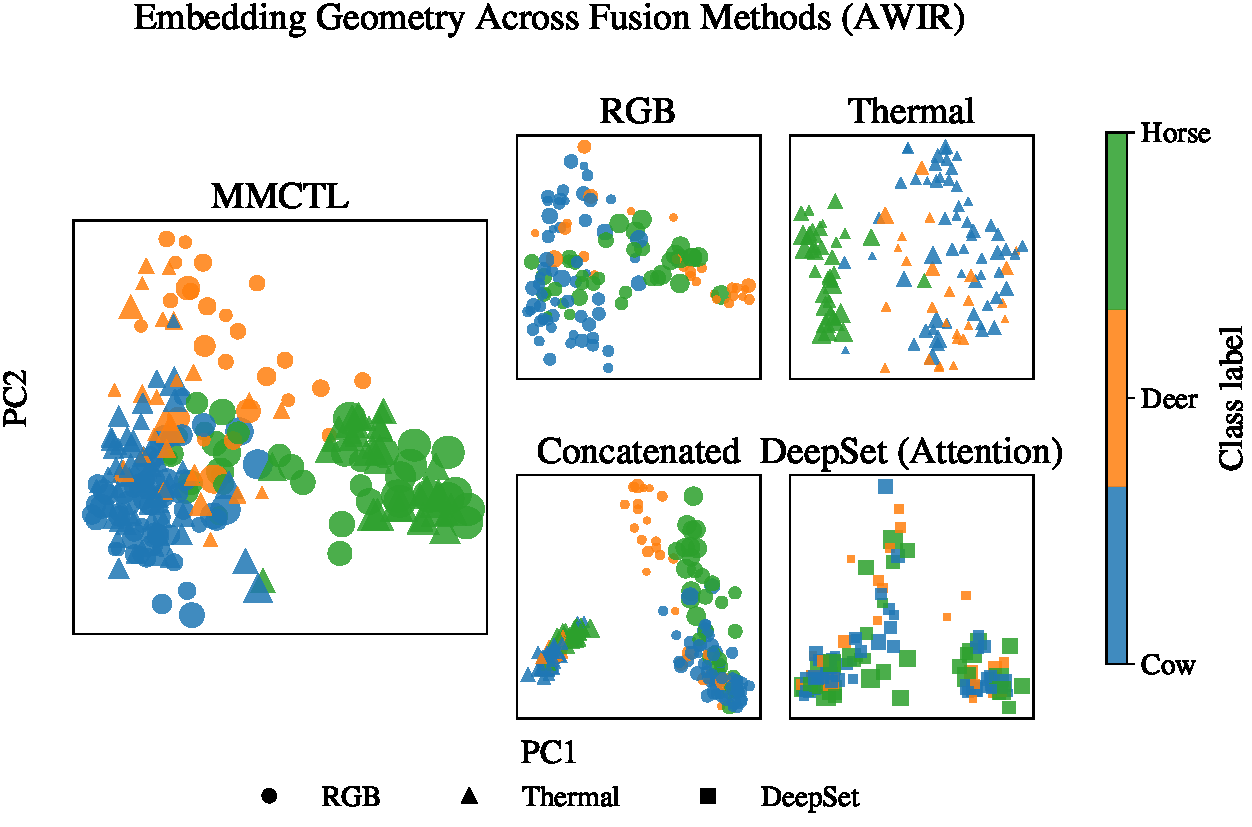
\includegraphics[width=\columnwidth]{figures/pca_highlight_mmctl_run01_double.pdf}
    \caption{Visualization of AWIR fused embeddings projected using PCA. Points are colored by class label and sized by bounding box area. MMCTL aligns RGB and thermal embeddings corresponding to the same objects while preserving semantic separation and continuous geometric variation.}
    \label{fig:emb_awir}
\end{figure}

\section{Methodology}
\label{sec:methodology}

\subsection{Problem Setup}
\label{subsec:problem-setup}

Consider a multi-modal dataset with $M$ sensing modalities and $N$ instances.
Let $\mathbf{x}_n^{(m)} \in \mathbb{R}^{d_m}$ denote the input for instance
$n \in \{1,\dots,N\}$ from modality $m \in \{1,\dots,M\}$, where $d_m$
denotes the modality-specific input dimensionality.

Each instance is associated with $T$ annotation sources.
For task $t \in \{1,\dots,T\}$, the annotation for instance $n$ is represented
by a row vector
\[
\mathbf{y}^{t}_{n}
=
\big[
y^{t}_{n,1}\;\; y^{t}_{n,2}\;\; \dots\;\; y^{t}_{n,L_t}
\big]
\in \mathbb{R}^{1 \times L_t},
\]
where $L_t$ denotes the number of annotation features for task $t$.

To ensure comparability across annotation sources with different scales,
each annotation feature is normalized independently to the interval $[0,1]$
using statistics computed from the training set only.
Let $\mathcal{N}_{\mathrm{train}} \subset \{1,\dots,N\}$ denote the index set of
training instances.

For each task $t$ and annotation feature index $\ell \in \{1,\dots,L_t\}$, define the
training-set extrema
\[
\mu^{t}_{\min,\ell}
=
\min_{n \in \mathcal{N}_{\mathrm{train}}} y^{t}_{n,\ell},
\qquad
\mu^{t}_{\max,\ell}
=
\max_{n \in \mathcal{N}_{\mathrm{train}}} y^{t}_{n,\ell}.
\]

\noindent Normalization is applied feature-wise as
\begin{equation}
\tilde{y}^{t}_{n,\ell}
=
\frac{
y^{t}_{n,\ell}
-
\mu^{t}_{\min,\ell}
}{
\mu^{t}_{\max,\ell}
-
\mu^{t}_{\min,\ell}
},
\qquad
\forall \ell \in \{1,\dots,L_t\}.
\end{equation}

\noindent The same normalization parameters are reused unchanged for validation and test instances. After normalization, annotation vectors are rescaled to account for differences in dimensionality across tasks.
Let
\[
L_{\max} = \max_{t \in \{1,\dots,T\}} L_t .
\]
Each normalized annotation vector is scaled and weighted as
\begin{equation}
\hat{\mathbf{y}}^{t}_{n}
=
w_t \, \tilde{\mathbf{y}}^{t}_{n}\, \frac{L_{\max}}{L_t},
\end{equation}
where $w_t \ge 0$ is a fixed hyperparameter controlling the influence of task $t$.

The final joint annotation vector for instance $n$ is constructed by horizontal
concatenation:
\begin{equation}
\mathbf{y}_{n}
=
\big[
\hat{\mathbf{y}}^{1}_{n}
\;\;
\hat{\mathbf{y}}^{2}_{n}
\;\;
\dots
\;\;
\hat{\mathbf{y}}^{T}_{n}
\big]
\in
\mathbb{R}^{1 \times L},
\end{equation}
where $L = \sum_{t=1}^{T} L_t$.
This joint annotation vector defines a unified similarity space whose geometry
reflects relationships across all annotation sources.


\subsection{Shared Latent Space with Modality-Specific Encoders}
\label{subsec:shared-latent-space}
Multi-modal observations provide complementary and non-redundant information about each instance, as different sensing modalities capture distinct physical, spectral, or geometric properties. Leveraging these complementary cues requires a representation that preserves modality-specific information while enabling direct comparison and alignment across modalities. To this end, each modality is processed by a dedicated encoder that maps modality-specific inputs into a shared latent space.

Each modality is processed by a dedicated encoder
$e_m(\cdot)$ that maps modality-specific inputs into a shared latent space.
For instance $n$ and modality $m$,
\begin{equation}
\mathbf{z}_n^{m}
=
e_m\!\left(\mathbf{x}_n^{m}\right),
\qquad
\mathbf{z}_n^{m} \in \mathbb{R}^{F},
\end{equation}
where $F$ denotes the shared embedding dimension.

Similarity in both annotation space and latent space is measured using cosine
distance,
\begin{equation}
D(\mathbf{u},\mathbf{v})
=
1 -
\frac{
\mathbf{u}^{\top}\mathbf{v}
}{
\|\mathbf{u}\|_2 \|\mathbf{v}\|_2
}.
\end{equation}

Triplets are formed using a batch-all strategy. For an anchor index $a$, all
pairs $(p,q)$ satisfying
\begin{equation}
D(\mathbf{y}_a,\mathbf{y}_p)
<
D(\mathbf{y}_a,\mathbf{y}_q)
\end{equation}
are included. This criterion defines relative similarity purely in annotation
space.

Let $K$ denote the number of valid triplets in a batch using a batch-all strategy. The multi-modal
adaptive triplet loss is
\begin{equation}
\begin{aligned}
\mathcal{L}_{\text{mm\_adaptive}}
=
\sum_{k=1}^{K}
\Big(
& \max\!\big(
D(\mathbf{z}_{a_k},\mathbf{z}_{p_k})^2
-
D(\mathbf{z}_{a_k},\mathbf{z}_{q_k})^2 \\
& \quad +
D(\mathbf{y}_{a_k},\mathbf{y}_{q_k})
-
D(\mathbf{y}_{a_k},\mathbf{y}_{p_k}),
\, 0
\big)
\Big).
\end{aligned}
\end{equation}

To encourage consistency between annotation-defined geometry and embedding
geometry, a regularization term enforces pairwise distance alignment,

\begin{equation}
\begin{aligned}
\mathcal{L}_{\text{mm\_reg}}
=
\sum_{k=1}^{K}
\Big(
& \left(
D(\mathbf{z}_{a_k},\mathbf{z}_{p_k})
-
D(\mathbf{y}_{a_k},\mathbf{y}_{p_k})
\right)^2 \\
& \quad +
\left(
D(\mathbf{z}_{a_k},\mathbf{z}_{q_k})
-
D(\mathbf{y}_{a_k},\mathbf{y}_{q_k})
\right)^2
\Big).
\end{aligned}
\end{equation}
The final Multi-Modal Continuous Triplet Loss is
\begin{equation}
\mathcal{L}_{\text{mm\_ctl}}
=
\mathcal{L}_{\text{mm\_adaptive}}
+
\mathcal{L}_{\text{mm\_reg}}.
\end{equation}

When the same instance is observed across multiple modalities, identical joint
annotation vectors yield zero annotation distance. This property encourages
embeddings of the same physical object from different sensing modalities to
align in the shared latent space while preserving continuous variation across
distinct instances.


\subsection{Modality-Specific Encoder Architecture}

Each sensing modality is first encoded using a dedicated convolutional autoencoder trained independently with a standard reconstruction objective. This design allows each encoder to specialize in extracting features aligned with the physical characteristics and information content of its corresponding modality, without imposing cross-modal constraints during representation learning.

For hyperspectral imagery, the encoder architecture emphasizes spectral feature extraction. The network uses $1 \times 1$ convolutions to model per-pixel spectral relationships, followed by densely connected layers that capture higher-order spectral interactions. Global average pooling is applied at the final convolutional stage to aggregate spectral responses into a fixed-length representation. For RGB, thermal, and LiDAR modalities, the encoder architecture emphasizes spatial structure. These encoders use spatial convolutions organized into dense blocks to capture local and contextual spatial patterns present in each modality. Global average pooling is applied after the final dense block to produce a compact representation that is invariant to spatial resolution.

In all cases, the encoder outputs a $1024$-dimensional latent embedding vector. After pretraining, encoder parameters are frozen and the resulting embeddings are used as fixed inputs for all fusion methods evaluated in this work. This separation ensures that differences in fusion performance reflect the quality of the shared latent organization rather than modality-specific feature learning. MMCTL trains modality-specific encoders and the shared latent space end-to-end using annotation-derived distance supervision, after which all embeddings are frozen and lightweight task heads are trained separately as shown in Fig. \ref{fig:MMCTL_Training_Architecture}.

\begin{figure}[!htb]
    \centering
    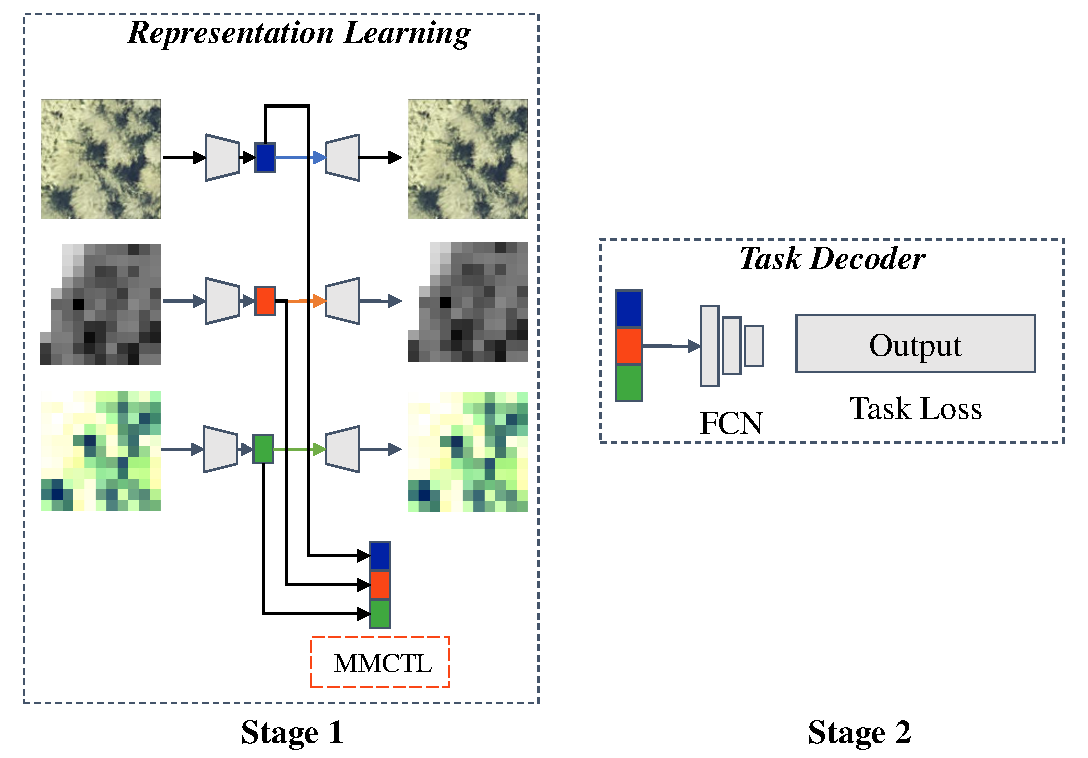
\includegraphics[width=\columnwidth]{figures/MMCTL-Framework-Figure.pdf}
    \caption{Two-stage MMCTL training on NEON. Modality-specific encoders are trained using multi-modal Continuous Triplet Loss with a shared annotation vector, then frozen while task-specific heads are trained independently to assess representation quality.}
    \label{fig:MMCTL_Training_Architecture}
\end{figure}

\section{Experiments}

\subsection{Datasets and Modalities}
\label{subsec:datasets}

Experiments are conducted on two remote sensing datasets that differ in sensing modalities, spatial resolution, and annotation structure. These datasets provide complementary test cases for evaluating multi-modal embedding fusion under heterogeneous sensing conditions.

The first dataset is Animal Wildlife Image Repository (AWIR) \cite{samiappan2024aerial, zhou2025multi}, which contains paired RGB and thermal imagery observing the same objects and spatial regions. RGB provides high-resolution visual appearance, while thermal supplies complementary temperature-based cues. The data processing follows the existing pipeline \cite{zhou2025multi}. The NEON dataset is derived from the NeonTreeEvaluation Benchmark \cite{Weinstein_Marconi_White_2022} and includes aligned RGB, hyperspectral, and LiDAR data from NEON airborne products. Tree crowns are centered on stem locations with species labels from NEON vegetation structure data \cite{NEON_vegetation_structure}. Species labels are provided per stem, crown polygons yield geometric attributes, and height statistics are computed from LiDAR-derived canopy height models, including minimum, maximum, mean, and standard deviation of height. We extract $6\times6$ patches at $1\,\mathrm{m}$ for hyperspectral and CHM and $60\times60$ patches at $10\,\mathrm{cm}$ for RGB, then apply Min-Max normalization using training statistics.

\subsection{Experimental Setup}
Evaluation targets embedding-level fusion under a two-stage protocol. For all comparison methods, modality-specific encoders are frozen and fusion operates on fixed embeddings. Task-driven fusion methods observe task labels directly during representation learning, while MMCTL relies solely on annotation-derived distance supervision (Section~\ref{subsec:shared-latent-space}). Datasets are split into $50\%$ training and $50\%$ test sets, with the test set excluded from model selection. $k$-fold cross-validation is applied within training, using $8$ folds for AWIR and $5$ folds for NEON. All splits use a fixed random seed, and results are reported as mean and standard deviation across folds. Categorical annotations use a fixed weight of $w_{\text{class}} = 0.5$ in the joint annotation vector for the AWIR dataset and $1.0$ for the NEON dataset to balance with continuous annotations.

Comparisons include concatenation and two DeepSet variants implemented with TorchMultimodal \cite{Facebookresearch}. Concatenation stacks modality embeddings and remains untrained. DeepSet fusion uses mean pooling \cite{reiter2020deep} or attention-based pooling and is trained with task-driven multi-task optimization. These methods contrast with MMCTL, which explicitly organizes latent geometry using annotation-derived similarity.

Next, task heads are optimized using supervised losses appropriate to each task, with identical architectures and optimization settings across all fusion methods. Training runs for up to $3000$ epochs with early stopping based on validation performance and a patience of $1000$ epochs. Optimization uses Adam with a learning rate of $10^{-3}$ and weight decay of $10^{-4}$. Batch size is set to $4$ for AWIR with no gradient clipping applied, while NEON uses a batch size of $32$ with gradient clipping enabled at a norm of $5$. Task heads use a shallow multilayer perceptron for both classification and regression tasks. Code for reproducing all experiments can be found at
\href{https://github.com/GatorSense/MMCTL}{github.com/GatorSense/MMCTL}.


\subsection{Latent Space Quality Metrics}
\label{sec:latent_space_quality_metrics}
Latent space structure is evaluated using simple global and local metrics that quantify alignment with annotation-defined geometry.

\paragraph{Global Consistency}
Let $\mathbf{z}_i \in \mathbb{R}^{d}$ denote the normalized embedding of sample $i$, and let $y_i^{(s)}$ denote the annotation for supervision source $s \in \{\mathrm{cls}, \mathrm{box}, \mathrm{pos}, \mathrm{height}\}$. For a pair $(i,j)$, embedding distance is $d_E(i,j) = \lVert \mathbf{z}_i - \mathbf{z}_j \rVert_2$, with annotation distance $d_s(i,j)$. Global consistency is
\begin{equation}
A_s
=
\mathbb{E}_{(i,j)}
\left[
\frac{d_E(i,j)}{d_s(i,j) + \epsilon}
\right],
\end{equation}
where lower values indicate stronger geometric alignment.

\paragraph{Local Smoothness}
Let $\mathcal{N}_k(i)$ denote the $k$ nearest neighbors of $\mathbf{z}_i$. Local smoothness is defined as
\begin{equation}
S_s(k)
=
\mathbb{E}_{i}
\left[
\operatorname{std}
\big(
\{ y_j^{(s)} : j \in \mathcal{N}_k(i) \}
\big)
\right],
\end{equation}
where lower values indicate greater annotation consistency among neighbors.

\paragraph{Structure Score}
For compact comparison, metrics are standardized across representations. The structure score is defined as
\begin{equation}
\mathrm{Struct}_s(k)
=
Z^{A}_s
+
Z^{S}_s(k),
\end{equation}
with lower values indicating stronger structure preservation. All experiments use $k=3$.

% Cosine distance is used during MMCTL training, while Euclidean distance is used for evaluation.



\subsection{Experimental Results}
Latent space structure is first evaluated using the global consistency and local smoothness metrics defined in Subsection~\ref{sec:latent_space_quality_metrics}. Table~\ref{tab:latent_alignment} compares structure scores across unimodal encoders, fusion methods, and MMCTL.

Across both datasets, standard fusion methods such as concatenation and DeepSet yield limited or inconsistent improvements over the strongest unimodal representations. While fusion can reduce variance, geometric alignment across supervision sources remains uneven. In contrast, MMCTL achieves the strongest latent structure for most annotations. On AWIR, MMCTL produces the best structure across all supervision sources, with large improvements relative to both unimodal and fusion methods. On NEON, MMCTL attains the strongest structure for box and height annotations and remains competitive for classification despite strong modality-specific baselines. These results indicate that annotation-driven multi-modal supervision yields more coherent and consistently aligned latent geometry than task-driven fusion strategies.


\newcommand{\err}[1]{\,\scriptstyle\pm\,\!#1}

\begin{table}[t]
\centering
\caption{
Latent space structure score across datasets. Two DeepSet (DS) methods are evaluated: Mean (M) and Attention (A). Annotation types include C for class labels, B for box, P for position, and H for height annotations.
}
\label{tab:latent_alignment}
\begin{tabular}{l c c c c}
\toprule
\textbf{Dataset} & \textbf{Method} 
& \textbf{C} $\downarrow$
& \textbf{B} $\downarrow$
& \textbf{P} $\downarrow$ \\
\midrule
\multirow{6}{*}{AWIR}
& RGB           
& $\phantom{-}0.43\err{0.28}$ 
& $-0.41\err{0.36}$ 
& $\phantom{-}0.23\err{0.38}$ \\
& Thermal       
& $\phantom{-}0.54\err{0.15}$ 
& $\phantom{-}0.56\err{0.14}$ 
& $\phantom{-}0.89\err{0.49}$ \\
\cmidrule(lr){2-5}
& Concat. 
& $-0.28\err{0.17}$ 
& $-0.19\err{0.15}$ 
& $\phantom{-}0.31\err{0.27}$ \\
& DS-A     
& $\phantom{-}1.17\err{0.44}$ 
& $\phantom{-}1.51\err{0.44}$ 
& $\phantom{-}1.19\err{0.43}$ \\
& DS-M       
& $\phantom{-}1.23\err{0.11}$ 
& $\phantom{-}1.47\err{0.46}$ 
& $\phantom{-}1.17\err{0.46}$ \\
\cmidrule(lr){2-5}
& MMCTL         
& $\mathbf{-3.10}\err{0.04}$ 
& $\mathbf{-2.93}\err{0.18}$ 
& $\mathbf{-3.79}\err{0.61}$ \\
\midrule
\multicolumn{2}{l}{}
& \textbf{C} $\downarrow$
& \textbf{B} $\downarrow$
& \textbf{H} $\downarrow$ \\
\midrule
\multirow{7}{*}{NEON}
& RGB           
& $\mathbf{-1.66}\err{0.88}$ 
& $-0.34\err{0.87}$ 
& $\phantom{-}0.48\err{0.97}$ \\
& HSI           
& $\phantom{-}0.72\err{0.11}$ 
& $\phantom{-}0.94\err{0.56}$ 
& $\phantom{-}1.49\err{0.23}$ \\
& LiDAR         
& $\phantom{-}2.60\err{0.08}$ 
& $\phantom{-}1.60\err{0.72}$ 
& $-0.35\err{0.17}$ \\
\cmidrule(lr){2-5}
& Concat. 
& $\phantom{-}0.39\err{0.15}$ 
& $\phantom{-}0.19\err{0.22}$ 
& $\phantom{-}0.36\err{0.05}$ \\
& DS-A     
& $-0.30\err{0.08}$ 
& $-0.56\err{0.48}$ 
& $-0.13\err{0.24}$ \\
& DS-M       
& $-0.27\err{0.12}$ 
& $\phantom{-}0.24\err{0.29}$ 
& $-0.27\err{0.23}$ \\
\cmidrule(lr){2-5}
& MMCTL         
& $-1.49\err{0.23}$ 
& $\mathbf{-2.07}\err{0.29}$ 
& $\mathbf{-1.58}\err{0.25}$ \\
\bottomrule
\end{tabular}
\end{table}

Table~\ref{tab:downstream_performance_tasks} reports downstream performance using frozen embeddings and highlights how MMCTL compares directly with state-of-the-art fusion strategies.

On AWIR, MMCTL surpasses the strongest fusion baselines across classification and both geometric regression tasks. DeepSet and concatenation improve semantic accuracy, yet gains in box and position regression remain limited. MMCTL delivers clearer improvements for geometric objectives while also achieving the highest classification performance. This pattern indicates that attention-based or additive fusion improves feature combination but does not sufficiently reorganize the latent space around continuous spatial structure. By enforcing annotation-consistent geometry during training, MMCTL yields a representation that generalizes more evenly across tasks when frozen.

On NEON, fusion methods provide a strong baseline by integrating complementary modality cues, particularly for classification and box regression. MMCTL nevertheless exceeds these approaches across all evaluated tasks. The largest gains appear in geometric objectives, where structured cross-modal alignment strengthens box and height prediction. Classification also improves, although by a smaller margin, reflecting the already strong semantic performance of advanced fusion methods. Despite heterogeneous modality relationships and resolution mismatch \cite{du2019multiresolution}, annotation-driven latent organization produces more transferable representations than fusion strategies focused primarily on discriminative integration.

Across both datasets, the comparison demonstrates that state-of-the-art fusion enhances feature integration but does not guarantee coherent annotation-aligned geometry. MMCTL extends beyond feature aggregation by explicitly structuring the latent space around joint semantic and geometric relationships. This structured organization translates into consistently stronger frozen-task generalization, which supports the broader claim that representation quality depends not only on modality combination but also on how the latent geometry is constrained during learning.

\begin{table}[t]
\centering
\caption{
Downstream task performance using unimodal and fused embeddings. Higher values indicate better performance. Annotation types include C for class labels, B for box, P for position, and H for height annotations.
}
\label{tab:downstream_performance_tasks}
\begin{tabular}{l c c c c}
\toprule
\textbf{Dataset} & \textbf{Method}
& \textbf{C (\%)} $\uparrow$
& \textbf{B $R^2$} $\uparrow$
& \textbf{P $R^2$} $\uparrow$ \\
\midrule
\multirow{6}{*}{AWIR}
& RGB        
& $77.08 \err{3.21}$ 
& $0.34 \err{0.07}$ 
& $-0.13 \err{0.16}$ \\
& Thermal    
& $78.96\err{1.59}$ 
& $0.30\err{0.07}$ 
& $-0.32 \err{0.34}$ \\
\cmidrule(lr){2-5}
& Concat.    
& $89.06 \err{1.44}$ 
& $0.32\err{0.08}$ 
& $-0.15 \err{0.20}$ \\
& DS-A  
& $87.71 \err{2.12}$ 
& $0.36\err{0.07}$ 
& $-0.18 \err{0.14}$ \\
& DS-M    
& $87.40 \err{1.51}$ 
& $0.37\err{0.05}$ 
& $-0.14 \err{0.15}$ \\
\cmidrule(lr){2-5}
& MMCTL      
& $\mathbf{94.06}\err{1.86}$ 
& $\mathbf{0.52}\err{0.07}$ 
& $\mathbf{0.12 }\err{0.08}$ \\
\midrule
\multicolumn{2}{l}{}
& \textbf{C (\%)} $\uparrow$
& \textbf{B $R^2$} $\uparrow$
& \textbf{H $R^2$} $\uparrow$ \\
\midrule
\multirow{7}{*}{NEON}
& RGB        
& $74.59\err{1.90}$ 
& $0.07 \err{0.15}$ 
& $0.34 \err{0.02}$ \\
& HSI        
& $76.69 \err{1.39}$ 
& $0.12 \err{0.08}$ 
& $0.40\err{0.05}$ \\
& LiDAR      
& $49.66 \err{1.15}$ 
& $0.22 \err{0.01}$ 
& $0.68 \err{0.02}$ \\
\cmidrule(lr){2-5}
& Concat.    
& $81.69 \err{1.08}$ 
& $0.39 \err{0.03}$ 
& $0.69 \err{0.02}$ \\
& DS-A  
% & $82.97 \err{1.03}$ 
& $83.65 \err0.88$ 
& $0.34 \err{0.09}$ 
& $0.61 \err{0.05}$ \\
& DS-M    
& $81.35 \err{1.18}$ 
& $0.40\err{0.01}$ 
& $0.61 \err{0.04}$ \\
\cmidrule(lr){2-5}  
& MMCTL      
& $\mathbf{86.95} \err{1.7}$ 
& $\mathbf{0.43} \err{0.04}$ 
& $\mathbf{0.74} \err{0.02}$ \\
\bottomrule
\end{tabular}
\end{table}


\subsection{Ablation Study}
An ablation study evaluates how varying the strength of semantic supervision influences the learned MMCTL representation on NEON. The classification annotation weight is varied from 0.5 to 2.0 in increments of 0.25, while the box and height annotation weights remain fixed at 1.0. This design isolates the impact of semantic weighting without modifying the contribution of geometric supervision. All models share identical architectures and hyperparameters across weight configurations so that observed differences arise exclusively from changes in classification emphasis. This controlled adjustment allows analysis of how increasing or decreasing semantic pressure reshapes the latent space while preserving consistent box and height structure.

\textbf{Results.} Fig.~\ref{fig:ablation2} shows that moderate classification weighting produces the strongest overall performance while extreme values introduce trade-offs. Classification improves as semantic weight increases from low values and stabilizes near a mid-range setting. Box regression follows a similar trend, peaking slightly above the balanced configuration before declining at higher weights, which suggests that excessive semantic emphasis begins to disrupt geometric structure. Height prediction remains comparatively stable across the entire range and consistently exceeds the SOTA baseline, indicating limited sensitivity to semantic weighting when geometric supervision is fixed. Overall, the results demonstrate that identifying the appropriate balance among annotation weights is a central challenge, as semantic and geometric supervision interact in ways that directly shape both discriminative and spatial structure within the MMCTL latent space.

\begin{figure}[!htb]
    \centering
    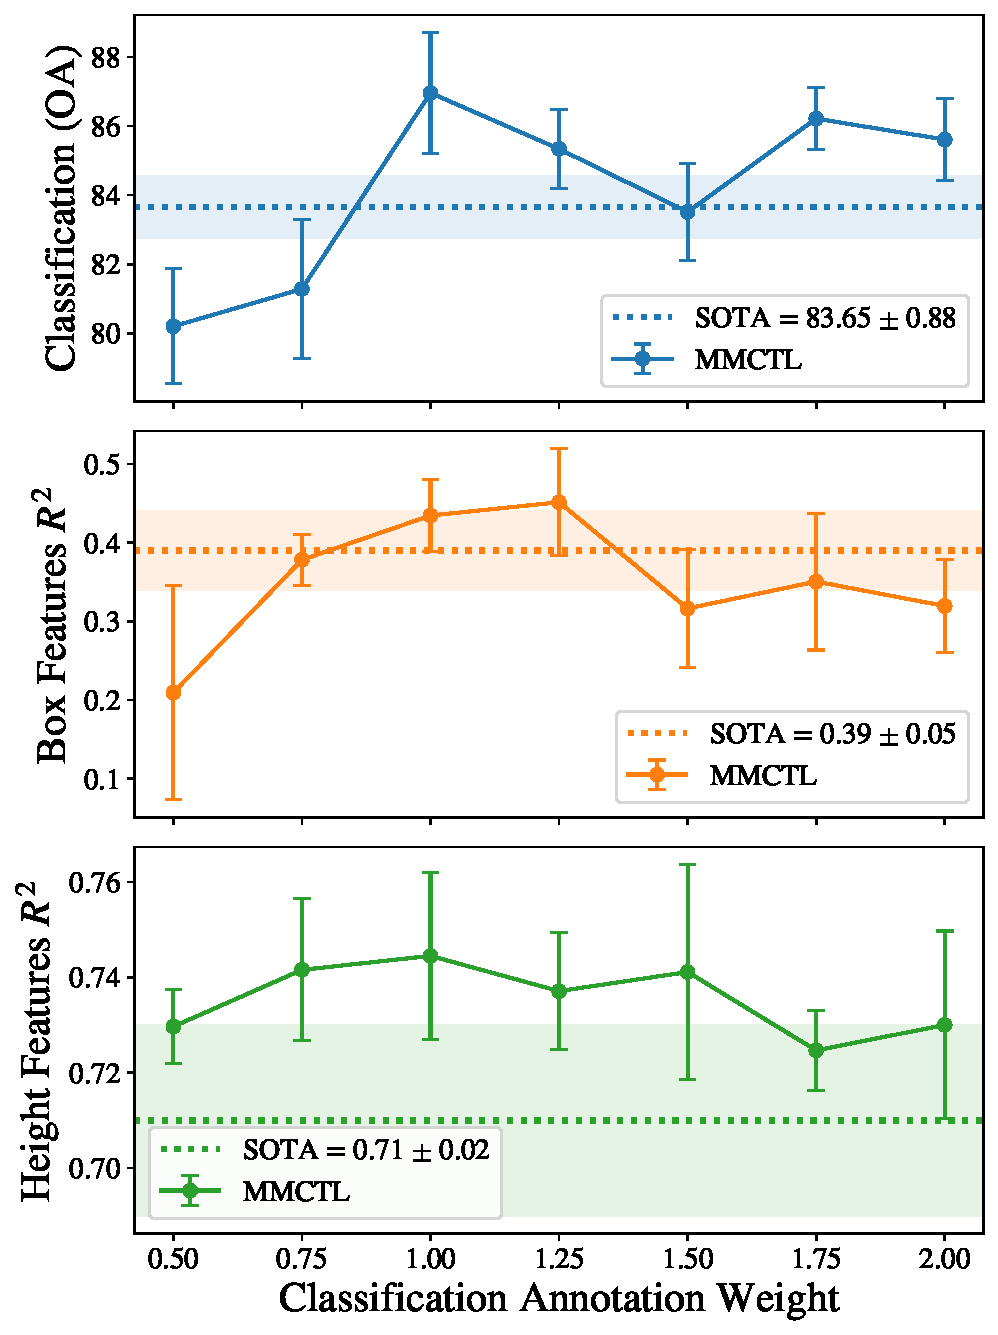
\includegraphics[width=\columnwidth]{figures/neon_task_eval_vs_class_weight.pdf}
    \caption{Task evaluation as a function of the classification annotation weight in MMCTL on the NEON dataset. The classification weight is varied from 0.5 to 2.0 while box and height weights remain fixed at 1.0. Dashed lines indicate SOTA performance with shaded regions representing standard deviation. Results are shown over the average of 5 runs.}
    \label{fig:ablation2}
\end{figure}

\section{Conclusion}
This work frames multi-modal representation learning as aligning embeddings across sensing modalities using annotation-defined similarity rather than task optimization. MMCTL builds a shared latent space by coupling modality-specific embeddings through weighted annotations, yielding more coherent cross-modal geometry than unimodal or task-driven fusion. Experiments on two datasets show that this structure may result in stronger downstream performance. Future work will explore learning annotation weights adaptively to allow the shared representation to respond to task relevance and modality strength.




\bibliographystyle{IEEEtran}
\bibliography{paper}




\vfill

\end{document}


